\documentclass[12pt]{article}

%Filter Warning messages, otherwise it would stuff like 
\usepackage{silence}
%Disable all warnings issued by latex starting with "You have..."
\WarningFilter{latex}{You have requested package}

%Allgemeine Einstellungen

%Abstände
\usepackage[a4paper,left=3cm,right=3cm,top=3cm,bottom=3.5cm,headsep=12pt]{geometry}%Bottom extra 0.5cm für Footer

%Deutsches Sprachpacket
\usepackage[german,ngerman]{babel}

%Times New Roman
\usepackage{mathptmx}

%Titelseite einbinden
\usepackage{pdfpages}

%1.5-Zeilenabstand
\usepackage[onehalfspacing]{setspace}

%Stil der Überschriften, siehe ueberschriften.sty
\usepackage[numeric]{../../ueberschriften}

%Stil des Inhaltsverzeichnisses, siehe inhaltsverzeichnis.sty
\usepackage[numeric]{../../inhaltsverzeichnis}

%Abkürzungsverzeichnis, siehe abk_verzeichnis.sty
\usepackage{../../abk_verzeichnis}

%Stil der Fußzeilen, siehe fusszeilen.sty
\usepackage{../../fusszeilen}

%Literaturverzeichnis und Zitate, siehe literatur.sty
\usepackage{../../literatur}

%Stil für Header und Footer, siehe header_footer.sty
%Wenn nicht erwünscht, müssen auch die Befehle \frontmatter, \mainmatter auskommentiert werden
\usepackage{../../header_footer}

%Stile für Code-Ausschnitte, siehe codes.sty
\usepackage{../../codes}

%Stile für Anhänge, Bilder, ...
\usepackage{../../anhang}

%Silbentrennung (manche Worte werden am Zeilenende nicht getrennt, diese müssen dann nachgetragen werden)
\usepackage[T1]{fontenc}
\hyphenation{öf-fent-lich-en}

%DEBUGGING (Zeigt Boxen an)
%\usepackage{showframe}
\setlength{\skip\footins}{12pt}

\usepackage{makecell}
\usepackage{placeins}

\begin{document}

\renewcommand{\mytitle}{Dokumentation/Tutorial}%Titel für oben links
\renewcommand{\myauthor}{Dr. Frank N. Furter}%Name für unten links

\begin{center}
\vspace*{2cm}
\LARGE{Vorlage für wissenschaftliches Arbeiten mit LaTeX\\[6pt]Dokumentation}
\end{center}

\clearpage

%
\includepdf[pages={1-}]{titelseite.pdf}

\frontmatter%Stil des Headers/Footers ändern

\pagenumbering{Roman}

\renewcommand{\plaintitle}{Inhaltsverzeichnis}%Titel für oben Rechts
%Defbox, damit gepunktete Linie bis zur Zahl geht
{\def\makebox[#1][#2]#3{#3}%
	\tableofcontents
}

\clearpage
\mainmatter%Stil des Headers/Footers ändern
\pagenumbering{arabic}

\part{Wie kann ich dieses Template benutzen?}

\section{Überschriften und Inhaltsverzeichnis}

\subsection{Wie kann ich Überschriften auf verschiedenen Ebenen erzeugen?}
Es können Überschriften auf 6 Ebenen erzeugt werden:
\begin{verbatim}
\part{Ebene 1}
\section{Ebene 2}
\subsection{Ebene 3}
\subsubsection{Ebene 4}
\paragraph{Ebene 5}
\subparagraph{Ebene 6}
\end{verbatim}

\noindent Wenn die Überschrift nicht nummeriert werden soll, muss der jeweilige Befehl mit einem * aufgerufen werden:
\begin{verbatim}
\section*{Ebene 1}
\end{verbatim}

\subsection{Wie kann ich die Nummerierung der Überschriften ändern?}
Die Überschriften können entweder nach einer rein nummerischen oder einer alphanummerischen Form nummeriert werden:
\begin{figure}[ht]
    \centering
    \begin{minipage}[t]{0.49\linewidth}
        \centering
        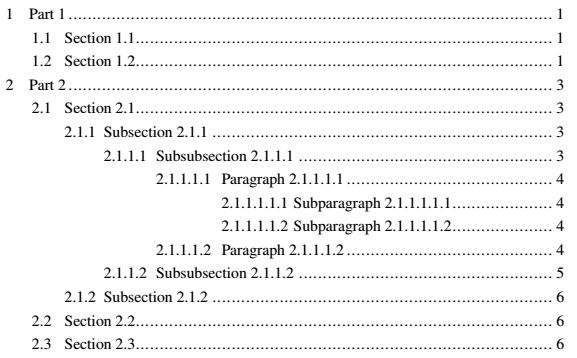
\includegraphics[width=\linewidth]{dokuImages/toc_num.png}
        \caption{numerisch}
    \end{minipage}% <- sonst wird hier ein Leerzeichen eingefügt
    \hfill
    \begin{minipage}[t]{0.49\linewidth}
        \centering
        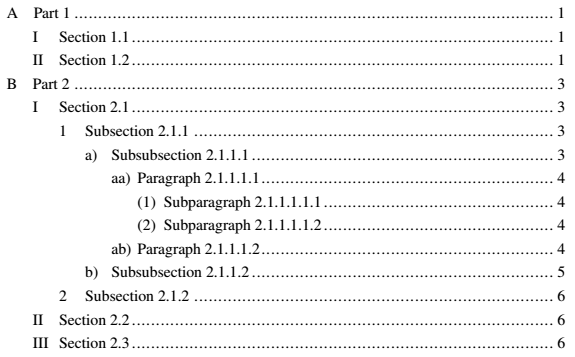
\includegraphics[width=\linewidth]{dokuImages/toc_alphanum.png}
        \caption{alpha-numerisch}
    \end{minipage}
\end{figure}
Der Wechsel erfolgt in der \textit{.tex}-Datei im Preämbel:\\[6pt]
Für numerisch:
\begin{verbatim}
\usepackage[numeric]{ueberschriften}
\usepackage[numeric]{inhaltsverzeichnis}
\end{verbatim}
Für alpha-numerisch:
\begin{verbatim}
\usepackage[latour]{ueberschriften}
\usepackage[latour]{inhaltsverzeichnis}
\end{verbatim}

\subsection{Wie kann ich es verhindern, dass für die oberste Ebene eine neue Seite gemacht wird?}
\begin{verbatim}
\partOnSamePage
\end{verbatim}

\subsection{Wie kann ich einen Eintrag zum Inhaltsverzeichnis hinzufügen?}
\begin{verbatim}
%Abk-Verz. ins Inhaltsverzeichnis
\addcontentsline{toc}{part}{Abkürzungsverzeichnis}
\end{verbatim}
Die Parameter sind das Element, zu dem hinzugefügt werde soll, die Ebene und der Titel.

\subsection{Wie kann ich das Inhaltsverzeichnis ausgeben?}
Um die gepunkteten Linien wirklich ganz bis zur Seitenzahl durchzuziehen, muss der Standard-Befehl noch in eine Box gewrappt werden:
\begin{verbatim}
{\def\makebox[#1][#2]#3{#3}%
	\tableofcontents
}
\end{verbatim}

\section{Abkürzungsverzeichnis}
Die Einträge im Abkürzungsverzeichnis werden automatisch aus der Datei \textit{abkuerzungen.csv} generiert. Dort sind sie in folgendem Format aufgeführt:
\begin{align*}
\text{abk}&;\text{bed};\\
\text{z.B.} &;\text{zum Beispiel};
\end{align*}
\noindent Um das Abkürzungsverzeichnis auf einer eigenen Seite auszugeben und auch im Inhaltsverzeichnis einzufügen:
\begin{verbatim}
\addcontentsline{toc}{part}{Abkürzungsverzeichnis}
\printabbreviations%abk_verzeichnis.sty
\clearpage
\end{verbatim}

\section{Bilder und Tabellen}
\subsection{Wie kann ich ein Bild im Text einbinden?}
\begin{verbatim}
\includegraphics[width=.9\textwidth]{./relativer/bildpfad.png}
\end{verbatim}

\subsection{Wie kann ich ein Bild im Abbildungsverzeichnis anzeigen?}
Um ein Bild im Abbildungsverzeichnis anzuzeigen, muss es in eine \textit{figure} gewrappt und mit einer Caption versehen werden:
\begin{verbatim}
\begin{figure}[ht]
    \centering
    \includegraphics[width=\linewidth]{relativer/bildpfad.png}
    \caption{Bild}
\end{figure}
\end{verbatim}
\noindent Die Option \textit{ht} gibt an, dass die Figure an diesem Ort stehen soll und nicht im Text fließen soll.

\section{Kopf- und Fußzeile}
Dieses Template bietet die Möglichkeit, folgende Informationen in Kopf- und Fußzeile anzuzeigen:
\begin{itemize}
\item oben-links: Titel der Arbeit
\item oben-rechts: aktueller Part (Überschrift Ebene 1)
\item unten-links: Autor
\item unten-rechts: Seite
\end{itemize}

\subsection{Wie kann ich den Titel und den Autor in der Kopf-/Fußzeile ändern?}
\begin{verbatim}
\renewcommand{\mytitle}{Dokumentation/Tutorial}%Titel für oben links
\renewcommand{\myauthor}{Dr. Frank N. Furter}%Name für unten links
\end{verbatim}
Bei einem Titel, der besser in zwei Zeilen passt, muss die Höhe der Kopfzeile angepasst werden:
\begin{verbatim}
\renewcommand{\mytitle}{Titel meiner Arbeit\\mit zwei Zeilen}
\renewcommand{\headheight}{27pt}
\end{verbatim}

\subsection{Wie kann ich den oben-rechts angezeigten Abschnitts-Titel ändern?}
Der Stil für die Header/Footer des Inhalts- und Literaturverzeichnisses sollen nicht auf den aktuellen Abschnittstitel zurückgreifen, sondern es soll der jeweilige Verzeichnisname angezeigt werden. Dieser wird in dem Befehl \textit{\textbackslash plaintitle} gespeichert/überschrieben. Die Art der Nummerierung kann ebenfalls gewechselt werden.
\begin{verbatim}
...

\frontmatter%Stil des Headers/Footers ändern

\pagenumbering{Roman}
...

\clearpage
\renewcommand{\plaintitle}{Abbildungsverzeichnis}
...

\clearpage
\renewcommand{\plaintitle}{Tabellenverzeichnis}
...

\clearpage
\renewcommand{\plaintitle}{Inhaltsverzeichnis}%Titel für oben Rechts
...

\clearpage
\mainmatter%Stil des Headers/Footers ändern

\part{Inhalt}
...

\clearpage
\frontmatter%Stil des Headers/Footers ändern
\renewcommand{\plaintitle}{Literaturverzeichnis}
\pagenumbering{Roman}
\setcounter{page}{5}
...
\end{verbatim}

\section{Literaturverzeichnis und Zitate}
LaTeX bietet zwar ein eigenes System zur Anzeige von Literatur an, darin sind Anpassungen aber sehr komplex/nicht so einfach umsetzbar. Deshab wurde für dieses Template ein eigenes System zur Literatur-Verwaltung entwickelt. Um dieses effektiv nutzen zu können, muss das Programm \textit{WA\_ LaTeX.exe} ausgeführt werden. Dies startet einen Webserver, welcher unter \textit{http://localhost:8081/overview} zu erreichen ist.

\subsection{Wie kann ich einen Literatur-Typen anlegen/bearbeiten?}
\begin{enumerate}
\item gehe auf \textit{http://localhost:8081/overview}
\item Klicke auf \textit{Neuen Typen erstellen}\newline
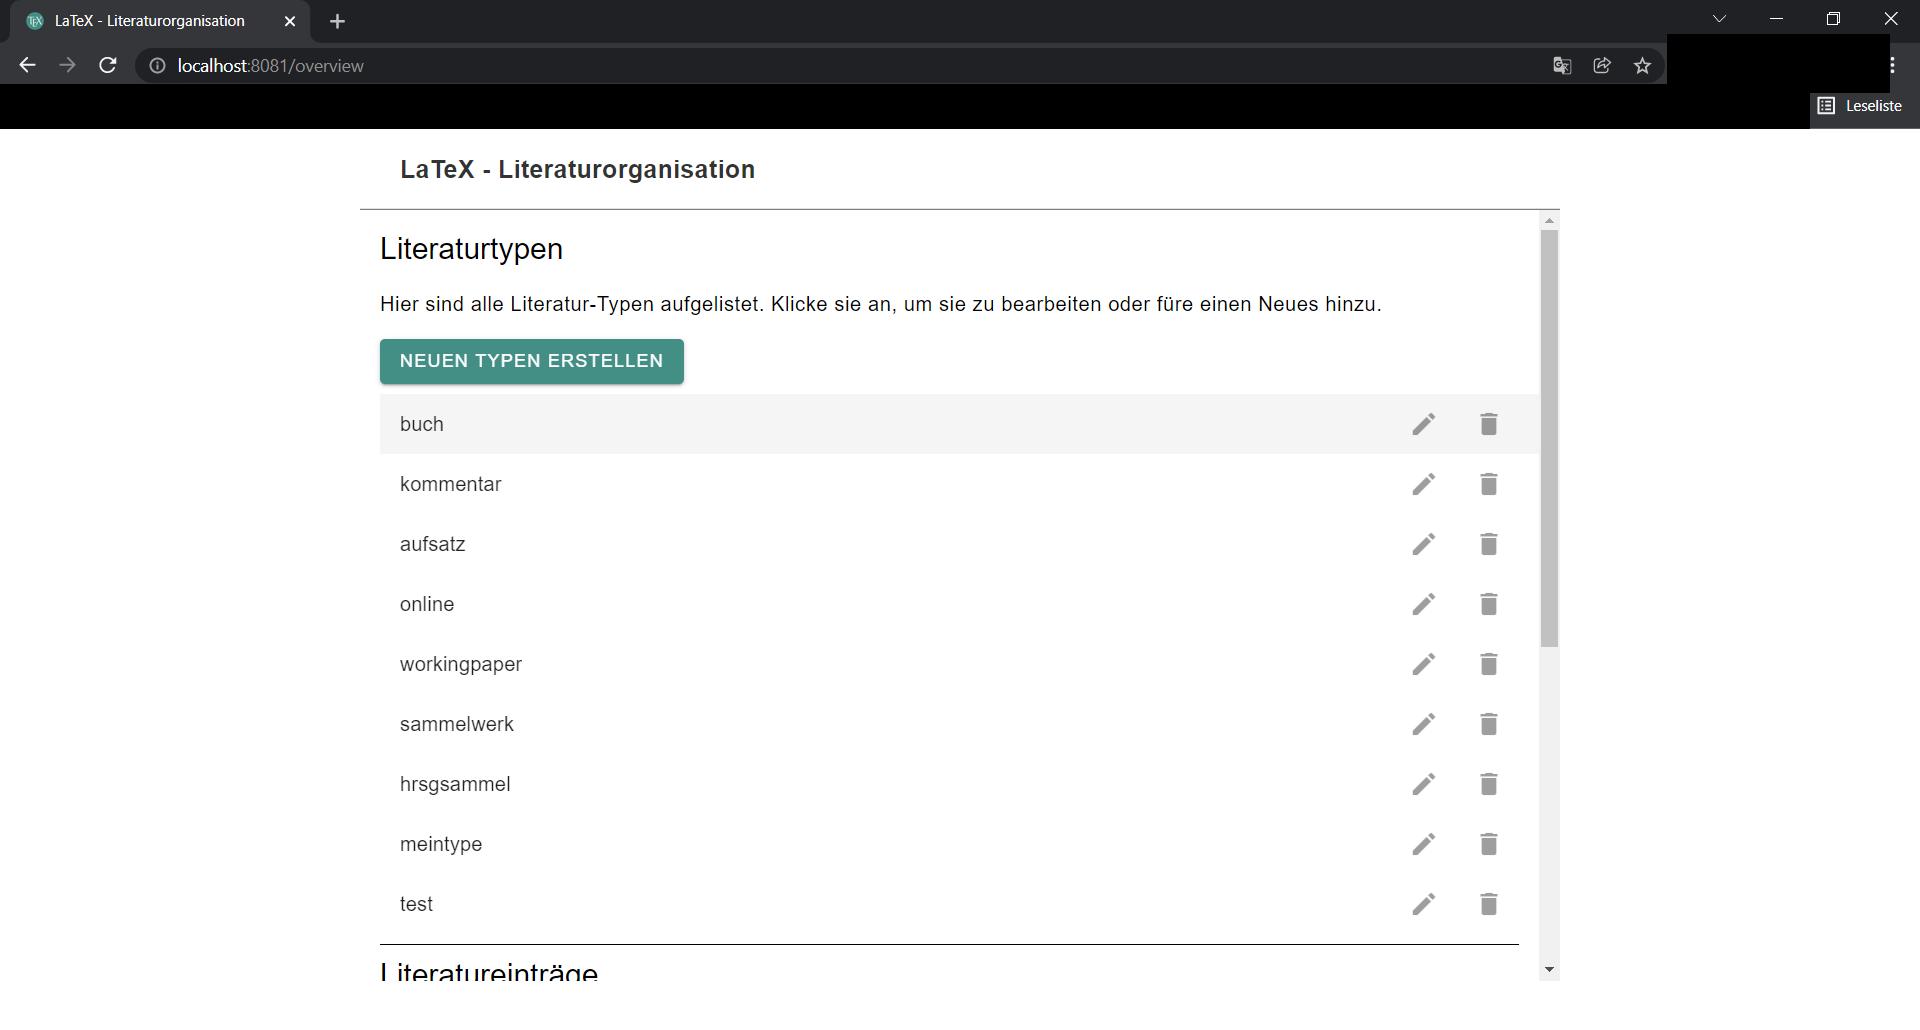
\includegraphics[width=\linewidth]{dokuImages/gui1_1.png}
\item gib einen Namen für den Literaturtyp an
\item Attribute fürs Literaturverzeichnis eingeben und stylen\\
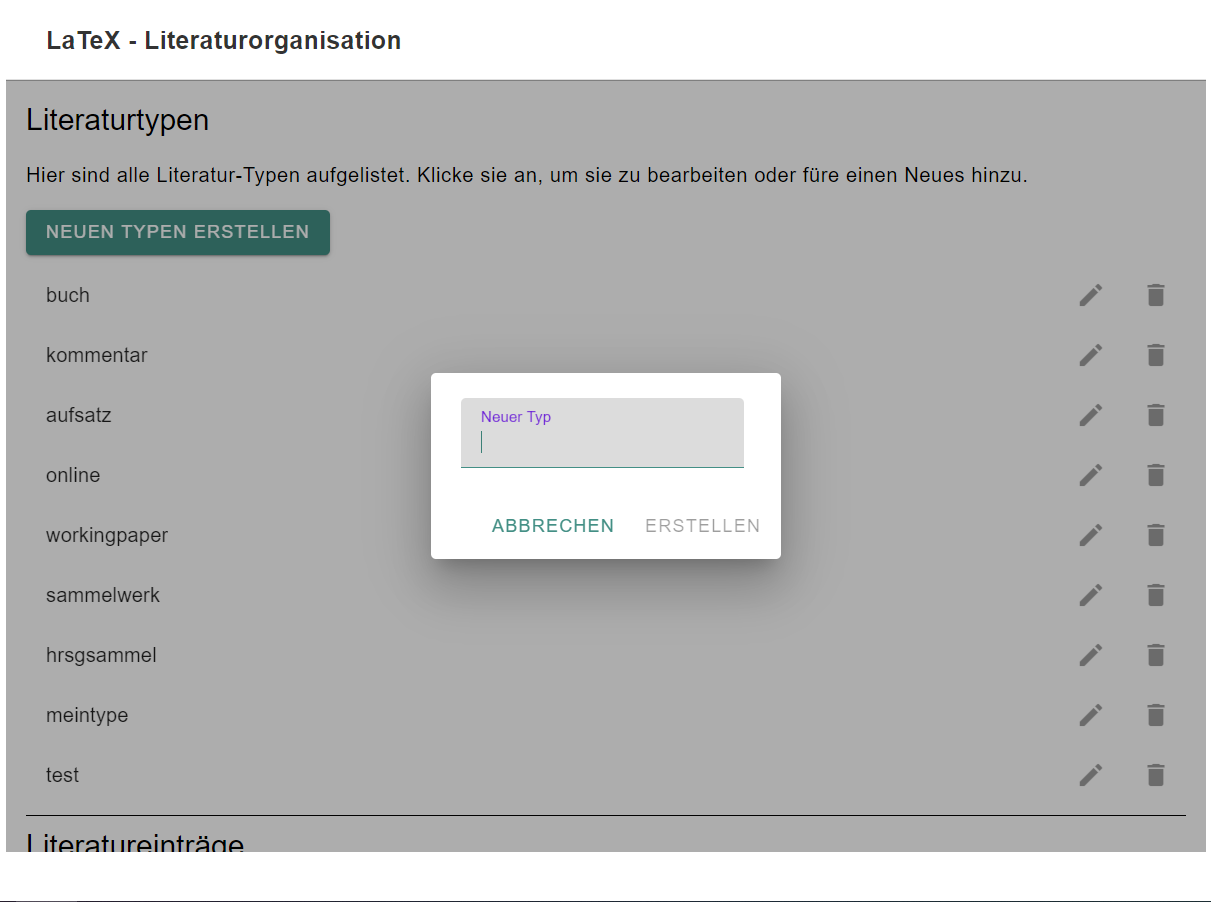
\includegraphics[width=\linewidth]{dokuImages/gui1_2.png}
\item Attribute für Zitate auswählen\\
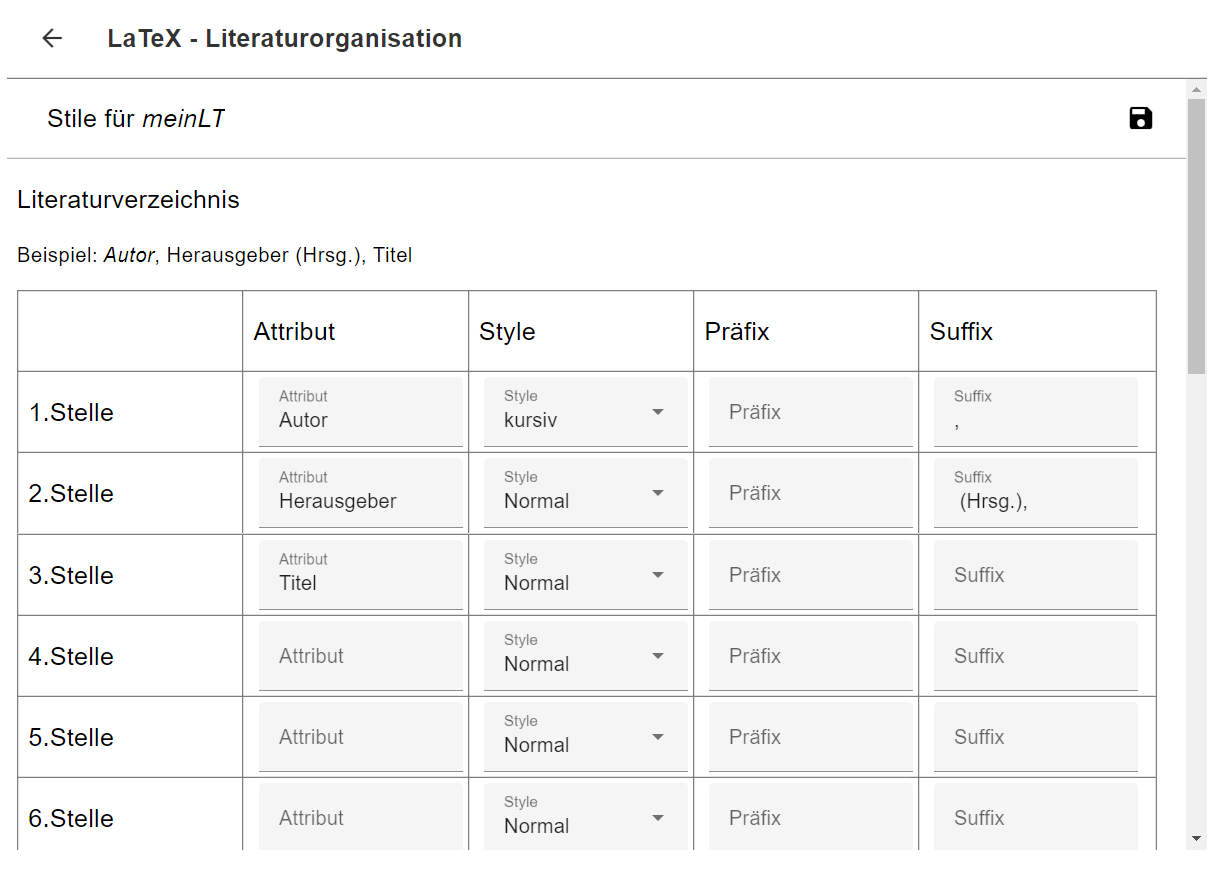
\includegraphics[width=\linewidth]{dokuImages/gui1_3.png}
\item Speichern
\item zum Bearbeiten oder Löschen einfach auf die Icons in der Liste klicken
\end{enumerate}

\subsection{Wie kann ich ein neues Projekt starten?}
\begin{enumerate}
\item gehe auf \textit{http://localhost:8081/overview}
\item Klicke auf \textit{Neues Projekt}
\item Gib einen Namen ein und klicke auf Speichern\newline
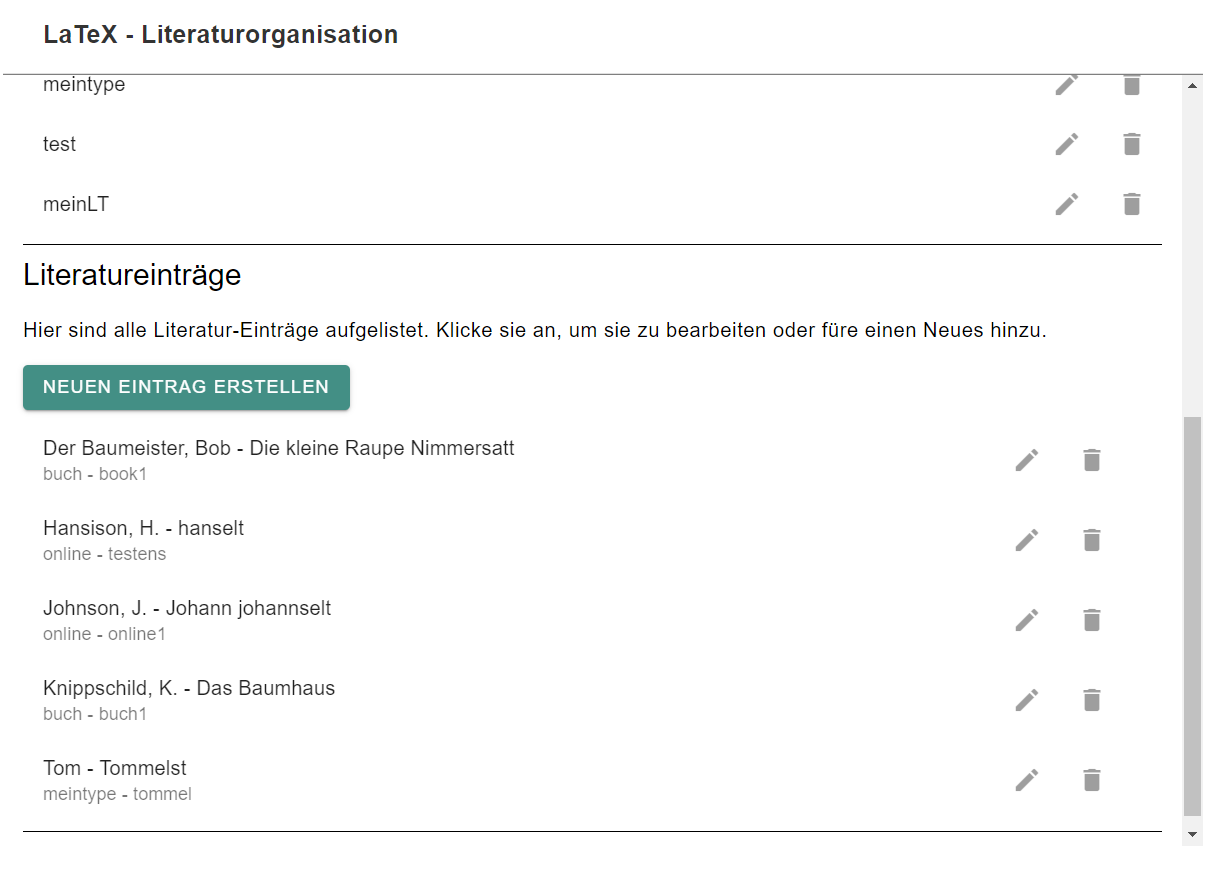
\includegraphics[width=\linewidth]{dokuImages/gui2_1.png}
\item Auf "Neuer Eintrag" klicken
\item Im Projekt eindeutigen Key eingeben, Typ auswählen und dann Attribute aufüllen\\
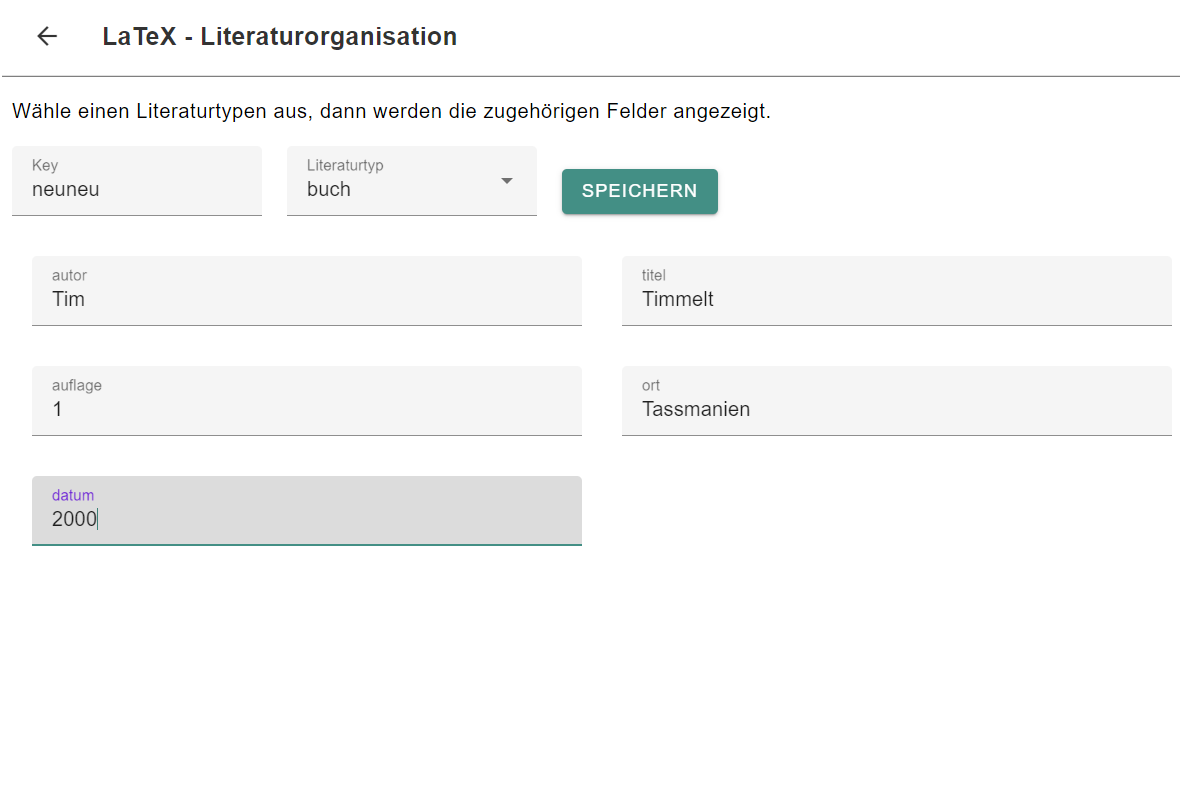
\includegraphics[width=\linewidth]{dokuImages/gui2_2.png}
\item Speichern
\item zum Bearbeiten oder Löschen einfach auf die Icons in der Liste klicken
\end{enumerate}

\subsection{Wir kann ich diesen erstellten Eintrag dann zitieren und im Literaturverzeichnis aufnehmen?}
Im Literaturverzeichnis wird automatisch alles aufgelistet.\\[6pt]Um die Quelle zu zitieren kann folgender Befehl im Text aufgerufen werden:
\begin{verbatim}
\citebib{KEY}{SEITEN}{Vgl.}
\end{verbatim}
Der zweite und dritte Parameter können leer bleiben.

\part{Häufig auftretende Fehler/Warnungen}
\section{Overfull hbox}
Manchmal ist der Inhalt zu breit, sodass rechts ein Überfluss entsteht. Um diesen zu erkennen, kann das Package \textit{showframe}  eingebunden werden.
\begin{verbatim}
%DEBUGGING (Zeigt Boxen an)
%\usepackage{showframe}
\end{verbatim}
Dies zeigt die Boxen von Header, Footer, Content und Seitenrand an.
\subsection{Silbentrennung}
Manchmal entsteht solch ein Überfluss, weil LaTeX die Silbentrennung nicht kennt. Dann kann dieses Wort im Preämel ergänzt werden:
\begin{verbatim}
\hyphenation{öf-fent-lich-en}
\end{verbatim}

\section{Invalid Character, missing \$ inserted, o.ä.}
Viele Sonderzeichen werden von LaTeX für Befehle verwendet und können deshalb nicht einfach so im Text verwendet werden. Man kann am besten googeln oder ausprobieren, einfach ein \textbackslash{} vor das Sonderzeichen zu setzen.

\section{Leerzeichen nach Sonderzeichen fehlt}
Entweder zwei Leerzeichen nach Sonderzeichen oder \textbackslash SONDERZEICHEN\{\}.

\section{Text eingeschoben}
Nach Bildern oder Tabellen ist Text ggf. eingeschoben. Um diesen Einschub zu entfernen muss vor dem Test \textit{\textbackslash noindent} eingefügt werden.

\section{Bilder und Tabellen fließen in Text}
Vor und nach dem Bild/der Tabelle muss eine \textit{Floatbarrier} eingefügt werden:
\begin{verbatim}
Text Text Text
\FloatBarrier
\begin{fiure}[ht]
...
\end{figure}
\FloatBarrier
Text Text Text
\end{verbatim}

\end{document}